\documentclass{article}
\usepackage{tikz}
\usetikzlibrary{positioning}

\begin{document}
\begin{center}
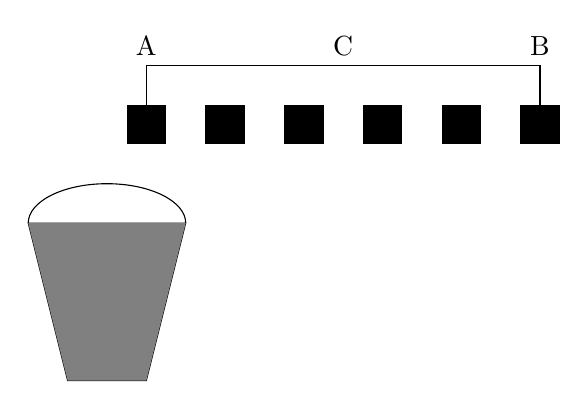
\begin{tikzpicture}

% definizione colore di riempimento
\tikzset{myfillcolor/.style ={fill=#1, draw=none}}
% definizione delle caratteristiche del nodo
\tikzset{mynode/.style={rectangle,draw, minimum width=0.5cm, minimum height=0.5cm}}

% Disegna dei nodi
\foreach \x in {0.5,1.5,...,5.5}
\node[mynode,myfillcolor=black] at (\x,0.75) {};

%Disegna linee
\draw (0.5,0.75)--(0.5,1.5)--(5.5,1.5)--(5.5,0.75);

%Metti un label sopra dei punti specifici delle linee disegnate
\foreach \t/\text in {{(0.5,1.5)/A},{(3,1.5)/C},{(5.5,1.5)/B}}
\node[above]at \t {\text};

%Traccia un arco
\draw (-1,-0.5) arc [start angle=180, end angle=0, x radius=1, y radius=0.5];
%Traccia il contorno di un oggetto a partire dai suoi vertici (--cycle) 
\draw (-1,-0.5) -- (-0.5,-2.5) -- (0.5,-2.5) -- (1,-0.5) --cycle;
%Se l'arco e il poligono sono disegnati al posto giusto puoi disegnare un secchio

%Riempi di un certo colore il poligono appena disengato
\fill[gray] (-1,-0.5) -- (-0.5,-2.5) -- (0.5,-2.5) -- (1,-0.5); 





\end{tikzpicture}
\end{center}
\end{document}
